%%%%%%%% ICML 2020 EXAMPLE LATEX SUBMISSION FILE %%%%%%%%%%%%%%%%%

\documentclass{article}

% Recommended, but optional, packages for figures and better typesetting:
\usepackage{microtype}
\usepackage{graphicx}
\usepackage{subfigure}
\usepackage{booktabs} % for professional tables
\usepackage{amsmath}
\usepackage{multirow}
\usepackage{xcolor}

% hyperref makes hyperlinks in the resulting PDF.
% If your build breaks (sometimes temporarily if a hyperlink spans a page)
% please comment out the following usepackage line and replace
% \usepackage{icml2020} with \usepackage[nohyperref]{icml2020} above.
\usepackage{hyperref}

% Attempt to make hyperref and algorithmic work together better:
\newcommand{\theHalgorithm}{\arabic{algorithm}}

% Use the following line for the initial blind version submitted for review:
\usepackage{icml2020}

% If accepted, instead use the following line for the camera-ready submission:
%\usepackage[accepted]{icml2020}

\newcommand\dmitry[1]{[\textcolor{red}{DS: {#1}}]}
\newcommand\yoav[1]{[\textcolor{blue}{YF: {#1}}]}
\newcommand\harsh[1]{[\textcolor{purple}{HM: {#1}}]}

% The \icmltitle you define below is probably too long as a header.
% Therefore, a short form for the running title is supplied here:
\icmltitlerunning{Quantifying Pointwise Stability}

\begin{document}

\twocolumn[
\icmltitle{Quantifying Pointwise Stability of Neural Networks}

\icmlsetsymbol{equal}{*}

\begin{icmlauthorlist}
\icmlauthor{Yoav Freund}{}
\icmlauthor{Harsh Mehta}{}
\icmlauthor{Dmitry Storcheus}{}
\end{icmlauthorlist}

\icmlaffiliation{to}{Department of Computation, University of Torontoland, Torontoland, Canada}
\icmlaffiliation{goo}{Googol ShallowMind, New London, Michigan, USA}
\icmlaffiliation{ed}{School of Computation, University of Edenborrow, Edenborrow, United Kingdom}

\icmlcorrespondingauthor{Cieua Vvvvv}{c.vvvvv@googol.com}
\icmlcorrespondingauthor{Eee Pppp}{ep@eden.co.uk}

% You may provide any keywords that you
% find helpful for describing your paper; these are used to populate
% the "keywords" metadata in the PDF but will not be shown in the document
\icmlkeywords{Machine Learning, ICML}

\vskip 0.3in
]

% this must go after the closing bracket ] following \twocolumn[ ...

% This command actually creates the footnote in the first column
% listing the affiliations and the copyright notice.
% The command takes one argument, which is text to display at the start of the footnote.
% The \icmlEqualContribution command is standard text for equal contribution.
% Remove it (just {}) if you do not need this facility.

%\printAffiliationsAndNotice{}  % leave blank if no need to mention equal contribution
\printAffiliationsAndNotice{\icmlEqualContribution} % otherwise use the standard text.

\begin{abstract}
\end{abstract}

\newtheorem{theorem}{Theorem}	

\newcommand{\cC}{{\cal C}}
\newcommand{\cD}{{\cal D}}
\newcommand{\cT}{{\cal T}}
\newcommand{\cN}{{\cal N}}
\newcommand{\cA}{{\cal A}}
\newcommand{\cE}{{\cal E}}
1\newcommand{\cH}{{\cal H}}
\newcommand{\cX}{{\cal X}}
\newcommand{\cY}{{\cal Y}}
\renewcommand{\Pr}[2]{\mbox{Pr}_{#1}\left[ #2 \right]}
\newcommand{\Hepsilon}{{\cal H}_{\epsilon}}

\newcommand{\paren}[1]{{\left({#1}\right)}}
\newcommand{\braces}[1]{{\left\{{#1}\right\}}}
\newcommand{\angles}[1]{{\left\langle{#1}\right\rangle}}
\newcommand{\abs}[1]{{\left|{#1}\right|}}
\newcommand{\floor}[1]{{\left\lfloor{#1}\right\rfloor}}
\newcommand{\brackets}[1]{{\left[{#1}\right]}}
\newcommand{\nextline}{\vspace{0.2cm}\\}   % a little space for equation arrays

\newcommand{\err}{\varepsilon}
\newcommand{\emperr}{\hat{\varepsilon}}
\newcommand{\lempir}{\hat{\ell}}
\newcommand{\ltrue}{\ell}
\newcommand{\pempir}{\hat{p}}
\newcommand{\ptrue}{p}
\newcommand{\lideal}{\ell}
\newcommand{\weight}{w}

\newcommand{\sign}{\mbox{\rm sign}}

\section{Motivation}
\label{sec:Motivation}

\begin{figure}[h]
\begin{center}
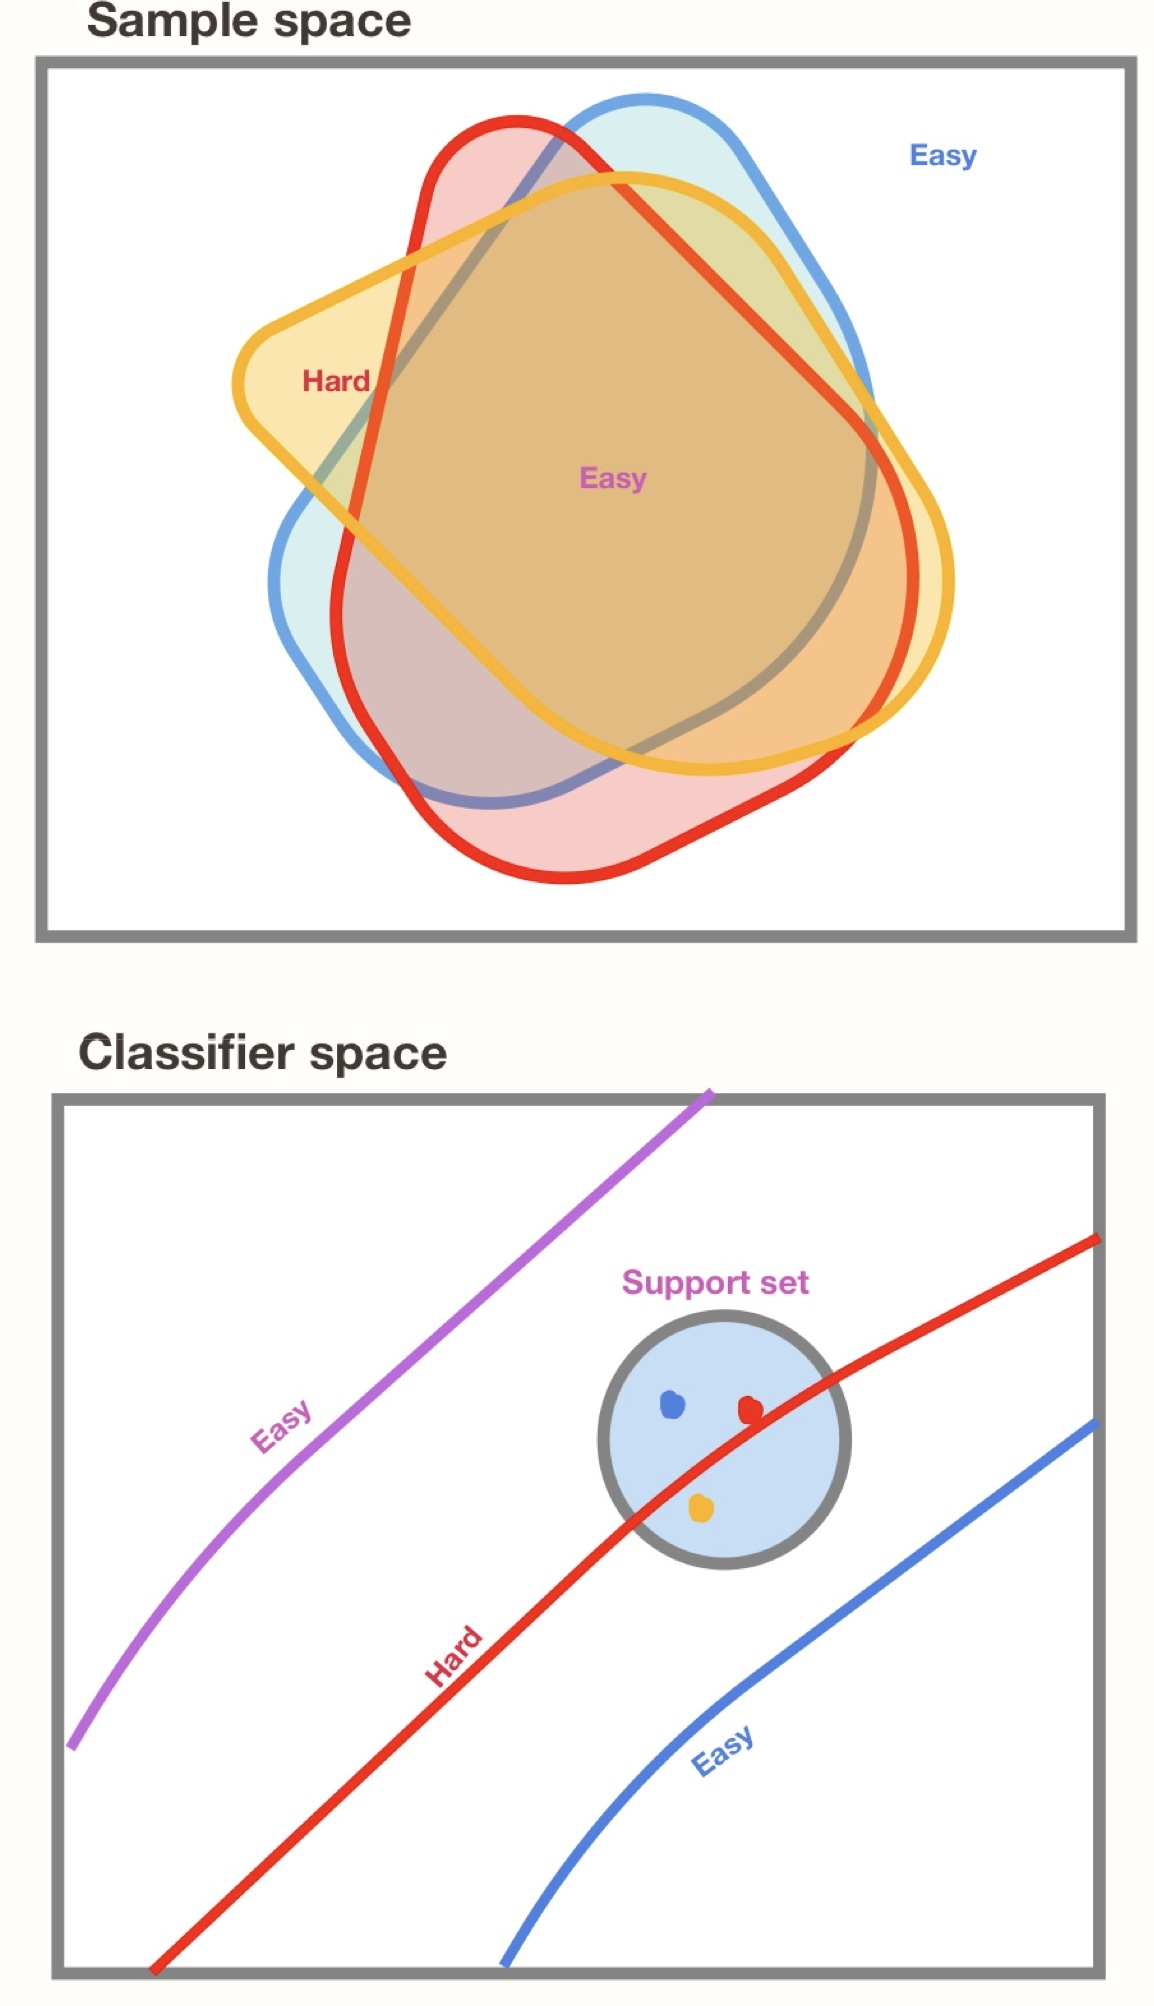
\includegraphics[width=2.5in]{figures/SupportSet.jpg}
\end{center}
\caption{{\bf support sets, easy and hard examples:} We use the dual
  relationship between binary classifiers and examples. We denote
  an instance by $x \in X$ and a classifier by $h \in \cH$. In the
  Instance space $X$ each point is an instance $x \in X$ and a
  classifier $h \in \cH$ defines a subset of $X$: $\{x |
  h(x)=1\}$. Similarly in the classifier space each point is an
  instance $h \in \cH$, and an instance defines a subset of $\cH$:
  $\{h | h(x)=1\}$. The three named points in the sample space
  correspond to
  the three boundaries in the classifier space with the matching
  colors. On the dual side, the three points in the classifier space
  correspond to the three sets in the example space.
\label{fig:duality}}
\end{figure}

One of the surprising phenomena of deep learning is that DNNs rarely
overfit. DNNs have been shown not to over-fit even when the number of
parameters is much larger than the number of examples.  This
phenomenon cannot be explained using structural measures of complexity
of the DNN, such as number of parameters or VC dimension. {\em
  Margins} based arguments have been used to explain the stability
when the data distribution is well matched to the
DNN~\cite{bartlett2017spectrally}.

 These analysis methods provide stability guarantees that are {\em
   global} in nature. The bounds proven using this approach are on the
 difference between the true error rate and the training or test error
 rates.  Global bounds can be used to bound the difference between the
 training error rate and the test error rate, which are global
 quantities. On the other hand, it provides no indicatin of where the
 errors are more likely to occur. In this paper we suggest a {\em local}
 stability measure which distinguishes between stable instances, on which our
 prediction can be confident, and unstable instances, on which our
 prediction is uncertain.

Our proposed algorithm follows the popular practice of independently training several DNNs and then combining them using a majority vote. Figure~\ref{fig:duality} is an intuitive explanation of the way the algorithm works in the binary case. The analysis is based on the interaction between two spaces: the sample space and the classifier space. We take advantage of the fact that the output of most learning algorithms, including DNNs, is sensitive to small changes in things such as reordering the training examples, changing the starting point, or bootstrapping the dataset.  We call the set of all classifiers that are likely to be generated the {\bf support set}. Each classifier in the support set defines a partitioning of the sample space into instances labeled +1 or -1. An instance is called {\bf easy} if all of the classifiers in the support set agree on it's label.  And example is called {\em hard} if about half of the classifiers in the support set predict +1 and half predict -1. 

It is well known that taking the majority vote over the classifiers in an ensemble improves robustness and accuracy. The novelty of our approach is that we use the majority vote only when the fractions of rules in the ensemble that predict +1 / -1 on and example is far from 50\%/50\%. when the number is close to 50\% / 50\% our classifier outputs "I don't know", which is represented as predicting with the set $\{-1,+1\}$. When classifying into more than two classes there are many different types of "I don't know". We adopt the idea of {\em set predictions} from the work Conformal Prediction~\cite{VovkConformalPrediction}.

Set predictions provide a detailed quantification of prediction uncertainty. Here are a few examples for when set predictions are useful.
\begin{itemize}
    \item {\bf Different costs for different mistakes:} for a self-driving car, it might be more important to determine whether an object is a human, less important to determine gender or age. Thus it is enough to determine whether the object is in the set \{man, woman, boy,girl\}. 
    \item {\bf Detection cascade:} Detecting the location and size of objects in video requires processing a rapid stream of candidate windows to detect a small fraction which contain the object. In their work on face detection~\cite{ViolaJones} Viola and Jones introduced the detection cascade as a method for reducing the {\em average} processing time by using a cascade of detectors, each filtering out windows that clearly contain no face. This can be expressed as predicting the sets \{not a face\} and \{a face, not a face\}.
    \item {\bf Many Classes:} When the number of classes is large, it can be useful to reduce the number of possibilities using a cascade: First stage identifies a subset, second stage reduces the subset, ... until a single class is determined. 
\end{itemize}



\iffalse
In this paper our focus is on the utility of pointwise
confidence. Consider first the standard case in which the training set
and test set are drawn from the same distribution. The ability to
distinguish between easy and hard examples creates useful options. For
example, by predicting on the easy examples while abstaining on the
hard examples the classifier can improve the classification
accuracy. In addition, abstaining on a binary label is more
informative than predicting $+1$ or $-1$ with equal probability, the
second hides the uncertainty, while abstaining reveals it.
\fi

{\bf Contributions:} Our main contribution is the use of an ensemble of NN to distinguish between stable and unstable instances. We develop the theoretical framework, extend it to the multi-class setup and demonstrate it's utility on CIFAR-10 and CIFAR-100.


\section{Comparison to other work}
\label{sec:OtherWork}
Not like calibration: does not depend on labels.

\section{Predicting with sets}

We use the notation $[K]$ to indicate the set of integers $\left\{
1,\ldots,K \right\}$.  Binary classification corresponds to $[2]$.
With binary classification, there is only one type of uncertainty to
consider, namely, uncertainty of whether the label is 0 or 1.  When
there are $K>2$ classes, there are many types of uncertainty. For
example, we might know that the label is 5 or 7, but not which of the
two. In order to represent these uncertainties we adopt the notion of
set predictions from Conformal Statistics~\cite{VovkConformalPrediction}. 

A set prediction is a subset of $[K]$, we denote the set of all
subsets of $[K]$ by $[[K]]$. Suppose $L \in [[K]]$ is a particular set
prediction, we say that the prediction is correct if the true label
$i$ is an element in $L$. If $|L|=1$ this amounts to a standard single
class prediction. At the other extreme, if $L=[K]$ the prediction is
always correct, and thus contains no useful information. The size $|L|$ is a tradeoff between
correctness, and informativity.

We adopt the convention that the output layer of the DNN consists of
$K$ units whose activations are non-negative and sum to 1, i.e. a
distribution, or a point on the $K$ dimensional simplex
$\Delta^K$. The standard mapping of the output $p \in \Delta$ to a
label is the index of a maximal coordinate in $p$.




\section{Support sets: definition and estimation}
\label{sec:SupportSet}

\newcommand{\sample}{\mbox{\bf sample}}
\newcommand{\start}{\mbox{\bf start}}
\newcommand{\order}{\mbox{\bf order}}
\newcommand{\cover}{\mbox{\bf cover}}

Learning algorithms are randomized. The first unavoidable source of
randomness is the choice of the training set, denoted $\sample$. DNNas
are usually trained using gradient-based methods. This results in two
additional sources of randomness: the choice of the starting point,
denoted $\start$ and the choice of the order of the training examples,
denote $\order$. Many other sources of randomness can be useful, here,
we restrict ourselfves to the three above plus an additional one that
will be defined for the sake of analysis.

In what follows we fix the architecture of the DNN. We denote by $w$
the weight vector of the DNN and by $W$ the space of all weight
vectors.  Let $R$ denote a source of randomness. We denote by $D^R$
the distribution over $W$ produced by $R$. 

We denote by
$w(x) \in \Delta^K$ the prediction of the network with weights $w$ on
the instance $x$.



Fixing $x$ and choosing the weight vector at random $w \sim D^R$
defines a distribution over $\Delta^K$ we denote by $D^R(x)$. 

The predictions of the ensemble $w_1(x),\ldots,w_m(x)$ can be interpreted as $m$ independent samples from $D^R(x)$

The predictions we use are subsets of $[K] = \{1,\ldots,K\}$. We denote this set of subsets by $[[K]]$.
We now define a mapping from the ensemble outputs $w_1(x),\ldots, w_m(x)$ to $[[K]]$.
The mapping is parametrized by a threshold $\theta \in [0,1]$. and defined as follows
(could be made into a figure):
\begin{enumerate}
  \item Let order 
\end{enumerate}

We denote the mean of this distribution by $\mu(x) \in \Delta^K$. We
define the ``ideal'' prediction as the set of maximal coordinates in
$\mu(x)$.
\[
p(x) = \left\{i \in [K] | \forall j \in [K], j \neq i,\; \mu(x)_i \geq \mu(x)_j\right\}
\]

Recall that $D^R(x)$ and $\mu(x)$ are not observable. The only
observable quantities are the predictions made by the ensemble members
$w_1(x),\ldots,w_k(x)$ which we can think of as samples from the
distribution $D^R(x)$ over $\Delta^K$.

We can formulate the 

\newcommand{\ens}{\mbox{ens}_m}



\iffalse
\section{Pseudo-Bayes Weighting}
\label{sec:Pseudo-Bayes}

Given an ensemble, we can identify the easiest examples - those
examples which are predicted the same way by all members of the
ensemble. We call these the ``unanimous-vote'' instances.
However, we are want to quantify the hardness of instances that are
not ``unanimous vote''. To do so we use a pseudo-Bayesian method
divised in~\cite{freund2004generalization} which we briefly describe here (for the binary
classification case).
Let $D$ be a fixed but unknown distribution over $(x,y)$ pairs, where
$x \in X$ and $y \in \{-1,+1\}$. 
Let $\cH$ be a fixed class of hypotheses, i.e., mappings from $X$ to
$\{-1,+1\}$.
Let $S$ denote a sample of $m$ training examples, each drawn independently
at random according to $D$.
We denote the {\em true} error of a hypothesis $h$ by
$\err(h) \doteq \Pr{(x,y) \sim D}{h(x) \neq y}$ and the estimated
error according to the sample $S$ by 
$\emperr(h) \doteq {1 \over m} \sum_{i=1}^m {\bf 1}\left[ h(x) \neq y
\right]$. 

The prediction algorithm that we study calculates for each hypothesis
$h$ a {\em weight} that is defined as
$
\weight(h) \doteq e^{-\eta \emperr(h)}
$
where $\eta>0$ is a parameter of the algorithm.
The prediction on a new instance $x$ is defined as a function of the
{\em empirical log ratio}:
\begin{eqnarray*}
\lempir_\eta(x) &\doteq &
{1 \over \eta}
\ln
\paren{\sum_{h, h(x)=+1} \weight(h)
 \over
 \sum_{h, h(x)=-1} \weight(h)
}\\
&=&
{1 \over \eta}
\ln
\paren{\sum_{h, h(x)=+1} e^{-\eta \emperr(h)}
 \over
 \sum_{h, h(x)=-1} e^{-\eta \emperr(h)}
}
~.
\end{eqnarray*} 
The prediction is defined to be
\begin{equation}  \label{eqn:prediction}
\pempir_{\eta,\Delta}(x) = 
\begin{cases}
\sign(\lempir(x))& \mbox{ if } |\lempir(x)|>\Delta \cr 
0 & \mbox{ otherwise }
\end{cases}
\end{equation}

where $\Delta \geq 0$ is a second parameter of the
algorithm.
Intuitively, the parameter $\Delta$ characterizes the range
of values of $\lempir_\eta(x)$ in which the training data is insufficient
to make a good prediction and a better choice is to abstain.
When clear from context, we generally drop the subscripts and write
simply $\lempir(x)$ and $\pempir(x)$.

A good tuning of these two parameters is $\eta = O(\sqrt{m})$ and
$\Delta = O(1/\sqrt{m})$. The formal statement is in the following theorem.

\begin{theorem}  \label{thm:1}
For any $\delta>0$ and $\eta>0$, if we set 
\[
\Delta = 2\sqrt{\ln(\sqrt{2}/\delta) \over m} + {\eta \over 8m}
\]
then, with probability at least $1-\delta$ over the random 
choice of the training set
\[
\Pr{(x,y) \sim D}{\pempir(x) \neq 0 \mbox{\rm ~and~}  
\pempir(x) \neq \sign(\ltrue(x))} \leq \delta.
\]
\end{theorem}

\fi

\section{The confidence-rated algorithm}

Putting all of this together, we arrive at the following algorithm:
\begin{enumerate}
\item {\bf Create ensemble:} Start with an empty ensemble and repeat
  until new classifiers are added only rarely:
  \begin{enumerate}
  \item Run a perturbation of the base learning algorithm to
    generate a classifier.
  \item If the classifier has at least $\epsilon$ disagreement with
    each of the classifiers in the ensemble, add it to the ensemble.
  \end{enumerate}
  \item {\bf weigh classifiers} each classifier in the ensemble
    according to $\weight(h) \doteq e^{-\eta \emperr(h)}$.
  \item {\bf Predict} the label of example $x$ to be $+1,?,-1$
    according to equation~(\ref{eqn:prediction})
\end{enumerate}


\section{Experimental Results}

\begin{tabular}{ |c|c|c|c|c| }
\hline
\multicolumn{5}{ |c| }{Error rates for different scoring methods} \\
\hline
\parbox[t]{1.5cm}{size of\\prediction set} &
\multicolumn{2}{c|}{\parbox[t]{1.5cm}{Margins}}&
\multicolumn{2}{c|}{\parbox[t]{1.5cm}{random \\ starting \\ points}}\\ \hline
& Incorrect & Correct & Incorrect & Correct \\ \hline
1 &  1.7 & 37.8 &  1.8 & 46.2 \\ \hline
2 &  1.2 & 18.7 &  2.5 & 26.1 \\ \hline
3 &  0.9 & 13.4 &  1.7 & 13.2 \\ \hline
4 &  0.7 & 10.6 &  0.8 &  5.5 \\ \hline
5 &  0.5 &  7.5 &  0.3 &  1.7 \\ \hline
6 &  0.2 &  4.0 &  0.0 &  0.3 \\ \hline
7 &  0.1 &  2.0 &  0.0 &  0.0 \\ \hline
8 &  0.0 &  0.7 &  0.0 &  0.0 \\ \hline
9 &  0.0 &  0.1 &  0.0 &  0.0 \\ \hline
10 &  0.0 &  0.0 &  0.0 &  0.0 \\ \hline
\end{tabular}


The results we have are for CIFAR which has 10 categories. The notion
of ``I don't know'' becomes complex.

We can overcome this by looking at particular pairs of labels,
some that are easy to discriminate and some that are harder. Another approach can be to partition the set of labels into two sets and distinguish between those.

In order to have publishable experiments on drifting, we need a good drifting dataset, preferably a binary one.

We might be able to report performance on Brand Safety. But I (yoav) find irreproducible results frustrating.

\begin{figure}[h]
\begin{center}
  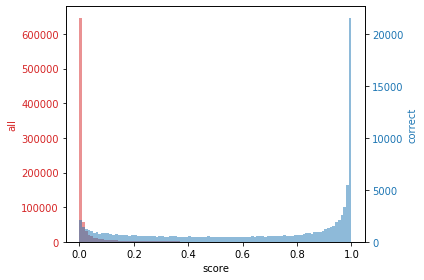
\includegraphics[width=3in]{figures/ScoreHist-unbounded.png}
  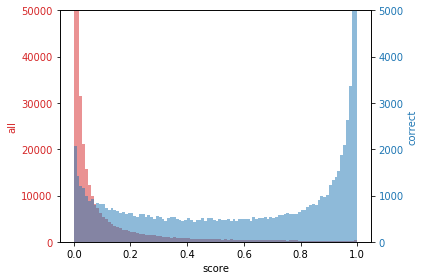
\includegraphics[width=3in]{figures/ScoreHist-Bounded.png}
\end{center}
\caption{{\bf Score Histograms}
\label{Histograms}}
\end{figure}

\begin{figure}[h]
\begin{center}
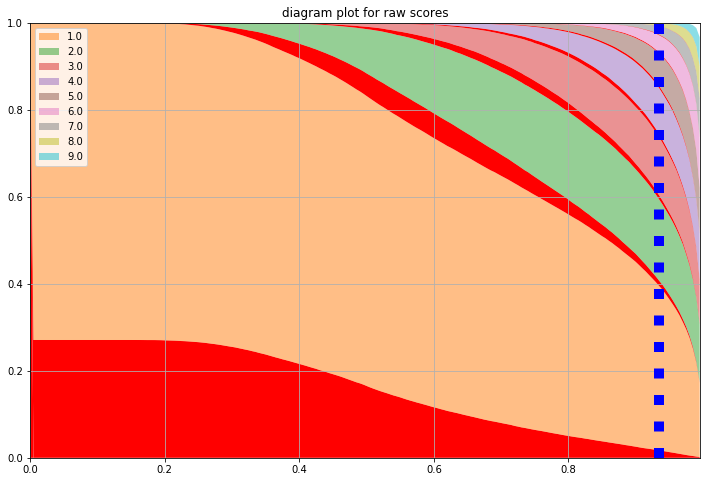
\includegraphics[width=3in]{figures/Margins.png}
\end{center}
\caption{{\bf Margins}
\label{fig:Margins}}
\end{figure}

\begin{figure}[h]
\begin{center}
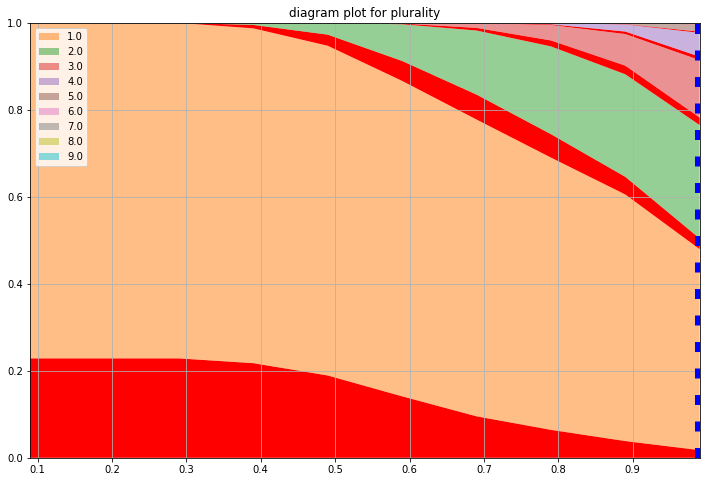
\includegraphics[width=3in]{figures/RandomStartEnsemble.png}
\end{center}
\caption{{\bf RandomStartEnsemble}
\label{fig:RandomStartEnsemble}}
\end{figure}

ScoreHist-unbounded.png

\bibliography{refs}
\bibliographystyle{icml2020}


%%%%%%%%%%%%%%%%%%%%%%%%%%%%%%%%%%%%%%%%%%%%%%%%%%%%%%%%%%%%%%%%%%%%%%%%%%%%%%%
%%%%%%%%%%%%%%%%%%%%%%%%%%%%%%%%%%%%%%%%%%%%%%%%%%%%%%%%%%%%%%%%%%%%%%%%%%%%%%%
% DELETE THIS PART. DO NOT PLACE CONTENT AFTER THE REFERENCES!
%%%%%%%%%%%%%%%%%%%%%%%%%%%%%%%%%%%%%%%%%%%%%%%%%%%%%%%%%%%%%%%%%%%%%%%%%%%%%%%
%%%%%%%%%%%%%%%%%%%%%%%%%%%%%%%%%%%%%%%%%%%%%%%%%%%%%%%%%%%%%%%%%%%%%%%%%%%%%%%
\appendix

%%%%%%%%%%%%%%%%%%%%%%%%%%%%%%%%%%%%%%%%%%%%%%%%%%%%%%%%%%%%%%%%%%%%%%%%%%%%%%%
%%%%%%%%%%%%%%%%%%%%%%%%%%%%%%%%%%%%%%%%%%%%%%%%%%%%%%%%%%%%%%%%%%%%%%%%%%%%%%%


\end{document}


